\begin{figure}[htbp]
    \centering
    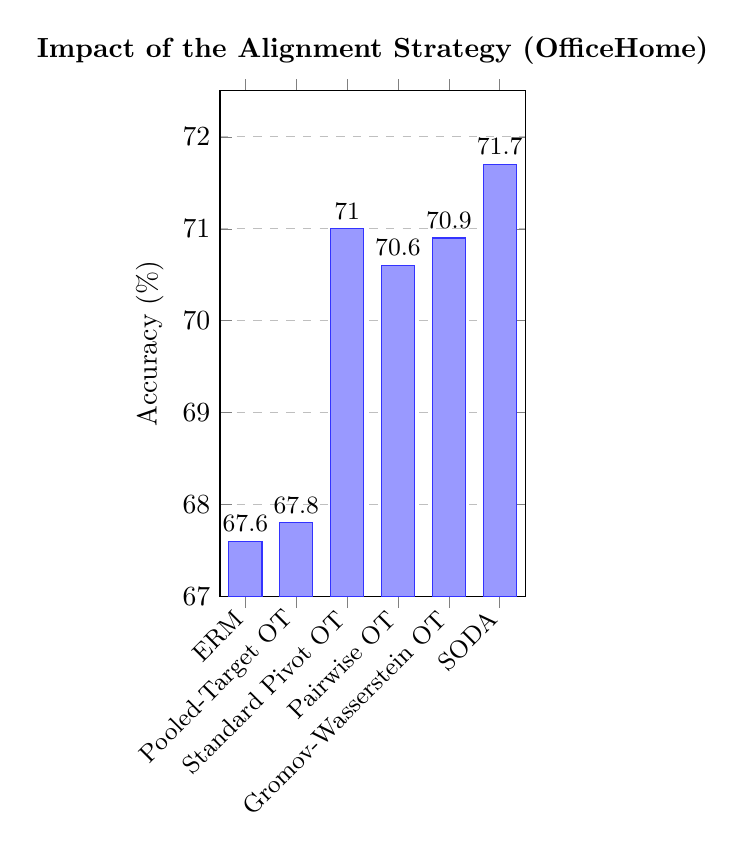
\begin{tikzpicture}
        \begin{axis}[
            % --- General Setup ---
            ybar,
            width=0.45\textwidth,
            height=8cm,
            bar width=12pt,
            % --- Titles and Labels ---
            title={\textbf{Impact of the Alignment Strategy (OfficeHome)}},
            ylabel={Accuracy (\%)},
            % --- X-Axis ---
            symbolic x coords={
                ERM,
                {Pooled-Target OT},
                {Standard Pivot OT},
                {Pairwise OT},
                {Gromov-Wasserstein OT},
                SODA
            },
            xtick=data,
            xticklabel style={
                rotate=45,
                anchor=east,
                font=\small
            },
            % --- Y-Axis Configuration ---
            ymin=67, 
            ymax=72.5,
            ymajorgrids=true,
            grid style=dashed,
            % --- Bar Labels ---
            nodes near coords,
            nodes near coords align={above},
            every node near coord/.append style={font=\small},
            % --- Layout and Spacing ---
            enlarge x limits=0.1,
        ]
        
        % --- Single addplot for all data points with a unified style ---
        \addplot[style={fill=blue!40, draw=blue!80}] table[x=x, y=y, col sep=comma] {
            x,                       y
            ERM,                     67.6
            {Pooled-Target OT},      67.8
            {Standard Pivot OT},     71.0
            {Pairwise OT},           70.6
            {Gromov-Wasserstein OT}, 70.9
            SODA,                    71.7
        };
        
        \end{axis}
    \end{tikzpicture}
    \caption{Effect of the alignment strategy on OfficeHome accuracy. SODA, with its stable DFR pivot, significantly outperforms the baseline ERM and all other OT-based strategies, including base approaches with unstable pivots and more advanced targets. This result highlights that a \textbf{stable pivot} is the critical component for effective alignment.}
    \label{fig:ablation_pivot_chart_final}
\end{figure}